\documentclass{article}
\usepackage{amsmath}
\usepackage{graphicx}
\usepackage{geometry}[margin=2cm]
\usepackage{example}
\usepackage{titlesec}
\usepackage{enumitem}

\begin{document}

\section*{Fitting Exercise 2 PHY224}
\subsection*{Hachem Fattouh}

In the second fitting exercise we are given seasonal data for the CO2 content
of the atmosphere for 100 years in parts per million (ppm). using a sinusoidal function with
a quadratic growth factor:

\[f(t) = at^2 + bt + c + d\sin{(2\pi t + \phi)} + e\sin{(4\pi t + \psi)}\]

with parameters \(a = 0.014, b = -53.21, c = 51620, d = 2.952, e = 0.8\bar{26}, \phi = 0.33, \psi = 2.211\),
the data can be approximated into a sinusoidal quadratic function as shown below

\begin{figure}[h]
    \centering
    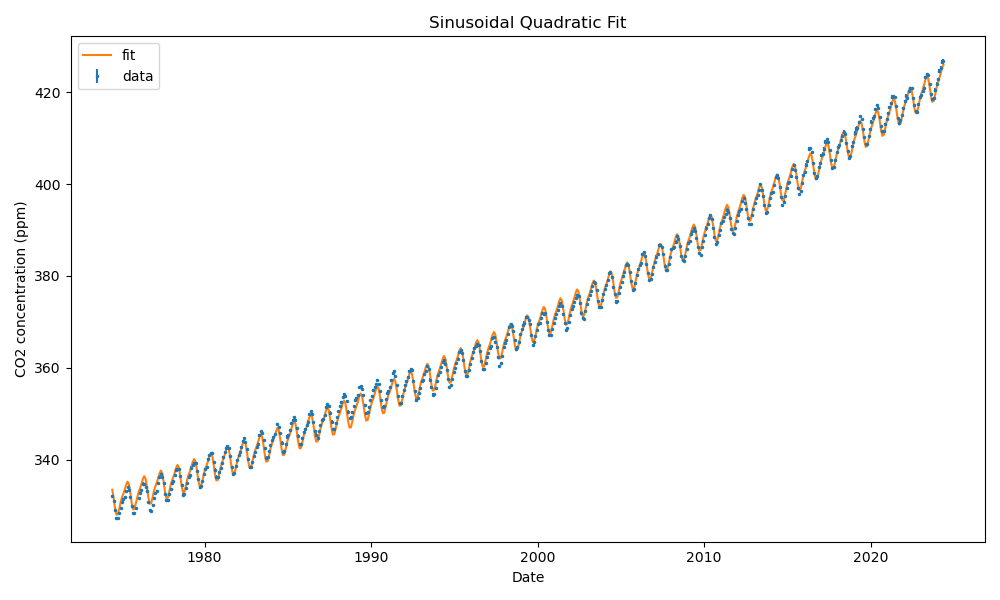
\includegraphics[width=\textwidth]{fitting_data_and_fit.png}
    \caption{Sinusoidal Quadratic Fit of CO2 Data}
    \label{fig:fit}
\end{figure}
\pagebreak

The residuals of this graph relative to the data are shown below.

\begin{figure}[h]
    \centering
    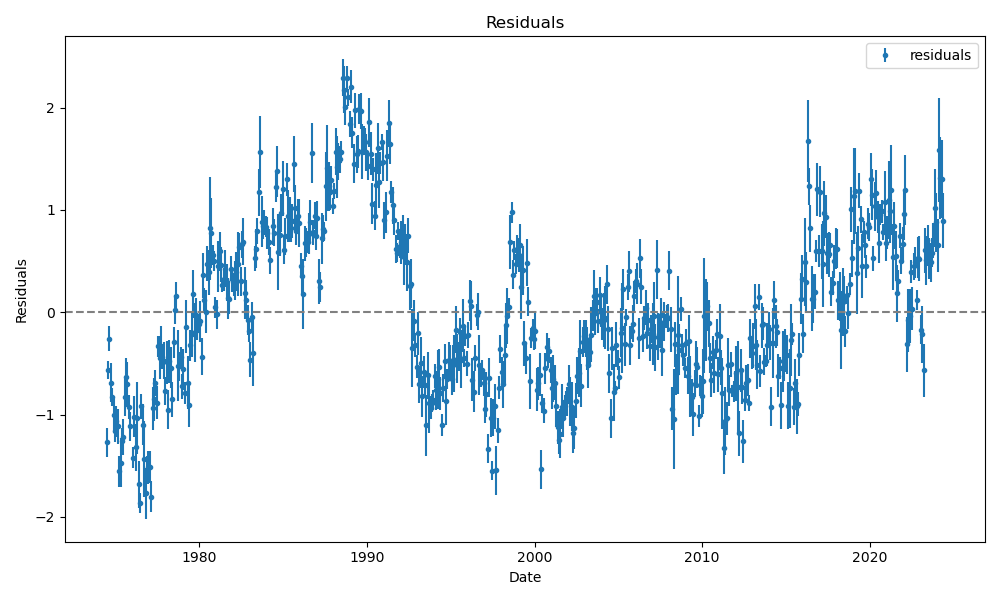
\includegraphics[width=\textwidth]{fitting_residuals.png}
    \caption{Residuals of the Fit}
    \label{fig:residuals}
\end{figure}

Using the data and these residuals, a \(\chi^2\) value of \(27.54\) is obtained
which is quite accurate to the data set, due to the reduced chi squared of around
0.034, which indicates high accuracy to the data-set, but could also indicate
an overfitted model. 

\pagebreak
\subsection*{Questions}

\begin{enumerate}[label=\alph*)]
    \item Which month has the highest CO\textsubscript{2} emissions? 
    does it change over time? how does this compare to the growing seasons on Earth?

    the month with the highest CO\textsubscript{2} emissions tends to occur at the end of the winter months,
    normally in May. it steadily rises to this peak from the beginning of the winter, and then slowly falls off
    to a trough in the summer, around september. this is mainly due to plants in the
    northern hemisphere dying and being snow covered, being less able to absorb atmospheric
    CO\textsubscript{2} during photosynthesis, among many other lesser factors at play.

    \item When will the predicted CO\textsubscript{2} models pass twice the 
    pre-industrial amount of 285ppm?

    some simple extra code to operate on the model indicates that this is going to happen 
    on 2071-09-24, or the 24th of September, 2071.

    \item how long will it take for the CO\textsubscript{2} maximum in 2000
    to be passed by the CO\textsubscript{2} minimum in the future.

    according to another addendum to the code linked, the date found here would be roughly
    october of 2022, which has already passed as of writing this.

\end{enumerate}

\end{document}